% Options for packages loaded elsewhere
\PassOptionsToPackage{unicode}{hyperref}
\PassOptionsToPackage{hyphens}{url}
%
\documentclass[
  10pt,
]{ctexart}
\usepackage{amsmath,amssymb}
\usepackage{iftex}
\ifPDFTeX
  \usepackage[T1]{fontenc}
  \usepackage[utf8]{inputenc}
  \usepackage{textcomp} % provide euro and other symbols
\else % if luatex or xetex
  \usepackage{unicode-math} % this also loads fontspec
  \defaultfontfeatures{Scale=MatchLowercase}
  \defaultfontfeatures[\rmfamily]{Ligatures=TeX,Scale=1}
\fi
\usepackage{lmodern}
\ifPDFTeX\else
  % xetex/luatex font selection
\fi
% Use upquote if available, for straight quotes in verbatim environments
\IfFileExists{upquote.sty}{\usepackage{upquote}}{}
\IfFileExists{microtype.sty}{% use microtype if available
  \usepackage[]{microtype}
  \UseMicrotypeSet[protrusion]{basicmath} % disable protrusion for tt fonts
}{}
\makeatletter
\@ifundefined{KOMAClassName}{% if non-KOMA class
  \IfFileExists{parskip.sty}{%
    \usepackage{parskip}
  }{% else
    \setlength{\parindent}{0pt}
    \setlength{\parskip}{6pt plus 2pt minus 1pt}}
}{% if KOMA class
  \KOMAoptions{parskip=half}}
\makeatother
\usepackage{xcolor}
\usepackage[margin=1in]{geometry}
\usepackage{color}
\usepackage{fancyvrb}
\newcommand{\VerbBar}{|}
\newcommand{\VERB}{\Verb[commandchars=\\\{\}]}
\DefineVerbatimEnvironment{Highlighting}{Verbatim}{commandchars=\\\{\}}
% Add ',fontsize=\small' for more characters per line
\usepackage{framed}
\definecolor{shadecolor}{RGB}{248,248,248}
\newenvironment{Shaded}{\begin{snugshade}}{\end{snugshade}}
\newcommand{\AlertTok}[1]{\textcolor[rgb]{0.94,0.16,0.16}{#1}}
\newcommand{\AnnotationTok}[1]{\textcolor[rgb]{0.56,0.35,0.01}{\textbf{\textit{#1}}}}
\newcommand{\AttributeTok}[1]{\textcolor[rgb]{0.13,0.29,0.53}{#1}}
\newcommand{\BaseNTok}[1]{\textcolor[rgb]{0.00,0.00,0.81}{#1}}
\newcommand{\BuiltInTok}[1]{#1}
\newcommand{\CharTok}[1]{\textcolor[rgb]{0.31,0.60,0.02}{#1}}
\newcommand{\CommentTok}[1]{\textcolor[rgb]{0.56,0.35,0.01}{\textit{#1}}}
\newcommand{\CommentVarTok}[1]{\textcolor[rgb]{0.56,0.35,0.01}{\textbf{\textit{#1}}}}
\newcommand{\ConstantTok}[1]{\textcolor[rgb]{0.56,0.35,0.01}{#1}}
\newcommand{\ControlFlowTok}[1]{\textcolor[rgb]{0.13,0.29,0.53}{\textbf{#1}}}
\newcommand{\DataTypeTok}[1]{\textcolor[rgb]{0.13,0.29,0.53}{#1}}
\newcommand{\DecValTok}[1]{\textcolor[rgb]{0.00,0.00,0.81}{#1}}
\newcommand{\DocumentationTok}[1]{\textcolor[rgb]{0.56,0.35,0.01}{\textbf{\textit{#1}}}}
\newcommand{\ErrorTok}[1]{\textcolor[rgb]{0.64,0.00,0.00}{\textbf{#1}}}
\newcommand{\ExtensionTok}[1]{#1}
\newcommand{\FloatTok}[1]{\textcolor[rgb]{0.00,0.00,0.81}{#1}}
\newcommand{\FunctionTok}[1]{\textcolor[rgb]{0.13,0.29,0.53}{\textbf{#1}}}
\newcommand{\ImportTok}[1]{#1}
\newcommand{\InformationTok}[1]{\textcolor[rgb]{0.56,0.35,0.01}{\textbf{\textit{#1}}}}
\newcommand{\KeywordTok}[1]{\textcolor[rgb]{0.13,0.29,0.53}{\textbf{#1}}}
\newcommand{\NormalTok}[1]{#1}
\newcommand{\OperatorTok}[1]{\textcolor[rgb]{0.81,0.36,0.00}{\textbf{#1}}}
\newcommand{\OtherTok}[1]{\textcolor[rgb]{0.56,0.35,0.01}{#1}}
\newcommand{\PreprocessorTok}[1]{\textcolor[rgb]{0.56,0.35,0.01}{\textit{#1}}}
\newcommand{\RegionMarkerTok}[1]{#1}
\newcommand{\SpecialCharTok}[1]{\textcolor[rgb]{0.81,0.36,0.00}{\textbf{#1}}}
\newcommand{\SpecialStringTok}[1]{\textcolor[rgb]{0.31,0.60,0.02}{#1}}
\newcommand{\StringTok}[1]{\textcolor[rgb]{0.31,0.60,0.02}{#1}}
\newcommand{\VariableTok}[1]{\textcolor[rgb]{0.00,0.00,0.00}{#1}}
\newcommand{\VerbatimStringTok}[1]{\textcolor[rgb]{0.31,0.60,0.02}{#1}}
\newcommand{\WarningTok}[1]{\textcolor[rgb]{0.56,0.35,0.01}{\textbf{\textit{#1}}}}
\usepackage{graphicx}
\makeatletter
\def\maxwidth{\ifdim\Gin@nat@width>\linewidth\linewidth\else\Gin@nat@width\fi}
\def\maxheight{\ifdim\Gin@nat@height>\textheight\textheight\else\Gin@nat@height\fi}
\makeatother
% Scale images if necessary, so that they will not overflow the page
% margins by default, and it is still possible to overwrite the defaults
% using explicit options in \includegraphics[width, height, ...]{}
\setkeys{Gin}{width=\maxwidth,height=\maxheight,keepaspectratio}
% Set default figure placement to htbp
\makeatletter
\def\fps@figure{htbp}
\makeatother
\setlength{\emergencystretch}{3em} % prevent overfull lines
\providecommand{\tightlist}{%
  \setlength{\itemsep}{0pt}\setlength{\parskip}{0pt}}
\setcounter{secnumdepth}{5}
\ifLuaTeX
  \usepackage{selnolig}  % disable illegal ligatures
\fi
\IfFileExists{bookmark.sty}{\usepackage{bookmark}}{\usepackage{hyperref}}
\IfFileExists{xurl.sty}{\usepackage{xurl}}{} % add URL line breaks if available
\urlstyle{same}
\hypersetup{
  pdftitle={加权线性回归R教程},
  pdfauthor={小狗},
  pdfkeywords={中文, R Markdown},
  hidelinks,
  pdfcreator={LaTeX via pandoc}}

\title{加权线性回归R教程}
\author{小狗}
\date{}

\begin{document}
\maketitle

{
\setcounter{tocdepth}{2}
\tableofcontents
}
\hypertarget{ux52a0ux6743ux7ebfux6027ux56deux5f52weighted-linear-regression}{%
\section{加权线性回归(Weighted Linear
Regression)}\label{ux52a0ux6743ux7ebfux6027ux56deux5f52weighted-linear-regression}}

\hypertarget{ux653eux5bbdux7ebfux6027ux6a21ux578bux7684ux5047ux8bbe}{%
\subsection{1.
放宽线性模型的假设}\label{ux653eux5bbdux7ebfux6027ux6a21ux578bux7684ux5047ux8bbe}}

\hypertarget{ux5e38ux89c4ux7ebfux6027ux56deux5f52ux6a21ux578bux7684ux5047ux8bbe}{%
\subsubsection{1.1
常规线性回归模型的假设}\label{ux5e38ux89c4ux7ebfux6027ux56deux5f52ux6a21ux578bux7684ux5047ux8bbe}}

在线性回归模型中,假设观测值 \(Y_i\) 与预测变量 \(x_i\)
的关系是线性的,模型形式如下:

\[
Y_i = x_i^T \beta + \epsilon_i
\]

其中: - \(Y_i\):第 \(i\) 个观测值的响应变量。 - \(x_i\):第 \(i\)
个观测值的预测变量(解释变量)的向量。 -
\(\beta\):回归系数向量,表示预测变量对响应变量的影响。 -
\(\epsilon_i\):误差项,表示实际观测值与模型预测值之间的差异。

误差项 \(\epsilon_i\) 的假设: 1. \textbf{零均值:}
\(E(\epsilon_i) = 0\),即误差的期望值为零。 2. \textbf{同方差性:}
\(\text{Var}(\epsilon_i) = \sigma^2\),所有观测点的误差方差相同。 3.
\textbf{独立性:} 各观测点的误差项相互独立。 4. \textbf{正态分布:}
\(\epsilon_i\) 服从正态分布 \(N(0, \sigma^2)\)。

\hypertarget{ux5f02ux65b9ux5deeux6027ux95eeux9898}{%
\subsubsection{1.2
异方差性问题}\label{ux5f02ux65b9ux5deeux6027ux95eeux9898}}

在某些应用中,观测点的误差方差可能不相等,这种现象称为\textbf{异方差性}。例如,某些数据点可能更可靠,应当赋予它们更大的权重。

\textbf{问题:}
如果继续使用普通最小二乘法(OLS)不考虑异方差性,结果可能会被方差较大的数据点影响,导致估计的不准确。

为了解决这一问题,\textbf{加权线性回归(WLS)}引入了权重,使得更可靠的观测值在模型中占据更大权重。

\begin{center}\rule{0.5\linewidth}{0.5pt}\end{center}

\hypertarget{ux52a0ux6743ux7ebfux6027ux56deux5f52ux7684ux5b9eux73b0}{%
\subsection{2.
加权线性回归的实现}\label{ux52a0ux6743ux7ebfux6027ux56deux5f52ux7684ux5b9eux73b0}}

在加权线性回归中,权重 \(w_i\) 是已知的、固定的,用来反映第 \(i\)
个观测点的重要性。模型的方差公式可以写成:

\[
\text{Var}(Y_i | x_i) = \frac{\phi}{w_i}
\]

权重 \(w_i\) 越大,观测点的方差越小,表明该观测值对回归模型更有信息量。

\hypertarget{ux6570ux636eux96c6ux51c6ux5907}{%
\subsubsection{2.1 数据集准备}\label{ux6570ux636eux96c6ux51c6ux5907}}

我们以风力发电机裂缝数据为例,假设每组发电机组运行一段时间后记录了裂缝比例。每组的数据权重(即发电机数量)不相同。

首先,生成数据集:

\begin{Shaded}
\begin{Highlighting}[]
\CommentTok{\# yi 表示每组风力发电机出现裂缝的比例}
\NormalTok{yi }\OtherTok{\textless{}{-}} \FunctionTok{c}\NormalTok{(}\FloatTok{0.00}\NormalTok{, }\FloatTok{0.08}\NormalTok{, }\FloatTok{0.06}\NormalTok{, }\FloatTok{0.10}\NormalTok{, }\FloatTok{0.17}\NormalTok{, }\FloatTok{0.23}\NormalTok{, }\FloatTok{0.21}\NormalTok{, }\FloatTok{0.46}\NormalTok{, }\FloatTok{0.65}\NormalTok{, }\FloatTok{0.52}\NormalTok{, }\FloatTok{0.58}\NormalTok{)}

\CommentTok{\# mi 表示每组发电机数量(作为权重)}
\NormalTok{mi }\OtherTok{\textless{}{-}} \FunctionTok{c}\NormalTok{(}\DecValTok{39}\NormalTok{, }\DecValTok{53}\NormalTok{, }\DecValTok{33}\NormalTok{, }\DecValTok{73}\NormalTok{, }\DecValTok{30}\NormalTok{, }\DecValTok{39}\NormalTok{, }\DecValTok{42}\NormalTok{, }\DecValTok{13}\NormalTok{, }\DecValTok{34}\NormalTok{, }\DecValTok{40}\NormalTok{, }\DecValTok{36}\NormalTok{)}

\CommentTok{\# 创建数据框}
\NormalTok{data }\OtherTok{\textless{}{-}} \FunctionTok{data.frame}\NormalTok{(yi, mi)}

\CommentTok{\# 打印数据集}
\FunctionTok{print}\NormalTok{(data)}
\end{Highlighting}
\end{Shaded}

\begin{verbatim}
##      yi mi
## 1  0.00 39
## 2  0.08 53
## 3  0.06 33
## 4  0.10 73
## 5  0.17 30
## 6  0.23 39
## 7  0.21 42
## 8  0.46 13
## 9  0.65 34
## 10 0.52 40
## 11 0.58 36
\end{verbatim}

\begin{center}\rule{0.5\linewidth}{0.5pt}\end{center}

\hypertarget{ux666eux901aux6700ux5c0fux4e8cux4e58ux6cd5olsux56deux5f52}{%
\subsection{3.
普通最小二乘法(OLS)回归}\label{ux666eux901aux6700ux5c0fux4e8cux4e58ux6cd5olsux56deux5f52}}

\hypertarget{ux666eux901aux6700ux5c0fux4e8cux4e58ux6cd5ux7684ux89e3ux91ca}{%
\subsubsection{3.1
普通最小二乘法的解释}\label{ux666eux901aux6700ux5c0fux4e8cux4e58ux6cd5ux7684ux89e3ux91ca}}

普通最小二乘法(OLS)的基本思想是最小化观测值与模型预测值之间的误差平方和。对于OLS回归,假设所有观测点的误差方差相等。

\textbf{OLS模型:}

\[
S(\beta) = \sum_{i=1}^{n} (y_i - x_i^T \beta)^2
\]

其中: - \(y_i\):第 \(i\) 个观测值。 - \(x_i^T \beta\):模型预测值。

OLS估计通过最小化误差平方和 \(S(\beta)\) 来估计参数 \(\beta\)。

\hypertarget{ols-ux6a21ux578bux7684ux5b9eux73b0}{%
\subsubsection{3.2 OLS
模型的实现}\label{ols-ux6a21ux578bux7684ux5b9eux73b0}}

在R中,我们可以通过\texttt{lm()}函数实现普通最小二乘法回归。由于数据集中只有一个常数项(即截距项),我们拟合一个常数模型。

\begin{Shaded}
\begin{Highlighting}[]
\CommentTok{\# OLS模型拟合}
\NormalTok{ols\_model }\OtherTok{\textless{}{-}} \FunctionTok{lm}\NormalTok{(yi }\SpecialCharTok{\textasciitilde{}} \DecValTok{1}\NormalTok{, }\AttributeTok{data =}\NormalTok{ data)}

\CommentTok{\# 输出OLS模型结果}
\FunctionTok{summary}\NormalTok{(ols\_model)}
\end{Highlighting}
\end{Shaded}

\begin{verbatim}
## 
## Call:
## lm(formula = yi ~ 1, data = data)
## 
## Residuals:
##      Min       1Q   Median       3Q      Max 
## -0.27818 -0.18818 -0.06818  0.21182  0.37182 
## 
## Coefficients:
##             Estimate Std. Error t value Pr(>|t|)   
## (Intercept)  0.27818    0.06978   3.987  0.00257 **
## ---
## Signif. codes:  0 '***' 0.001 '**' 0.01 '*' 0.05 '.' 0.1 ' ' 1
## 
## Residual standard error: 0.2314 on 10 degrees of freedom
\end{verbatim}

\hypertarget{ux53efux89c6ux5316olsux62dfux5408ux7ed3ux679c}{%
\subsubsection{3.3
可视化OLS拟合结果}\label{ux53efux89c6ux5316olsux62dfux5408ux7ed3ux679c}}

我们可以绘制OLS模型的拟合结果,将数据点和OLS拟合的常数(截距)显示出来:

\begin{Shaded}
\begin{Highlighting}[]
\CommentTok{\# 绘制OLS模型拟合结果}
\FunctionTok{plot}\NormalTok{(data}\SpecialCharTok{$}\NormalTok{yi, }\AttributeTok{main=}\StringTok{"OLS模型拟合"}\NormalTok{, }\AttributeTok{xlab=}\StringTok{"样本编号"}\NormalTok{, }\AttributeTok{ylab=}\StringTok{"裂缝比例"}\NormalTok{, }\AttributeTok{pch=}\DecValTok{19}\NormalTok{, }\AttributeTok{col=}\StringTok{"blue"}\NormalTok{)}
\FunctionTok{abline}\NormalTok{(}\AttributeTok{h=}\FunctionTok{mean}\NormalTok{(data}\SpecialCharTok{$}\NormalTok{yi), }\AttributeTok{col=}\StringTok{"red"}\NormalTok{, }\AttributeTok{lwd=}\DecValTok{2}\NormalTok{, }\AttributeTok{lty=}\DecValTok{2}\NormalTok{) }\CommentTok{\# OLS拟合水平线}
\FunctionTok{legend}\NormalTok{(}\StringTok{"topleft"}\NormalTok{, }\AttributeTok{legend=}\FunctionTok{c}\NormalTok{(}\StringTok{"观测点"}\NormalTok{, }\StringTok{"OLS拟合"}\NormalTok{), }\AttributeTok{col=}\FunctionTok{c}\NormalTok{(}\StringTok{"blue"}\NormalTok{, }\StringTok{"red"}\NormalTok{), }\AttributeTok{pch=}\FunctionTok{c}\NormalTok{(}\DecValTok{19}\NormalTok{, }\ConstantTok{NA}\NormalTok{), }\AttributeTok{lty=}\FunctionTok{c}\NormalTok{(}\ConstantTok{NA}\NormalTok{, }\DecValTok{2}\NormalTok{))}
\end{Highlighting}
\end{Shaded}

\begin{center}\rule{0.5\linewidth}{0.5pt}\end{center}

\hypertarget{ux52a0ux6743ux6700ux5c0fux4e8cux4e58ux6cd5wlsux56deux5f52}{%
\subsection{4.
加权最小二乘法(WLS)回归}\label{ux52a0ux6743ux6700ux5c0fux4e8cux4e58ux6cd5wlsux56deux5f52}}

\hypertarget{ux52a0ux6743ux6700ux5c0fux4e8cux4e58ux6cd5ux7684ux89e3ux91ca}{%
\subsubsection{4.1
加权最小二乘法的解释}\label{ux52a0ux6743ux6700ux5c0fux4e8cux4e58ux6cd5ux7684ux89e3ux91ca}}

加权最小二乘法(WLS)通过为每个观测点分配一个权重
\(w_i\),解决异方差性问题。权重越大,观测点的方差越小,对模型的贡献越大。WLS的目标是最小化加权的误差平方和:

\[
S(\beta) = \sum_{i=1}^{n} w_i (y_i - x_i^T \beta)^2
\]

\hypertarget{wls-ux6a21ux578bux7684ux5b9eux73b0}{%
\subsubsection{4.2 WLS
模型的实现}\label{wls-ux6a21ux578bux7684ux5b9eux73b0}}

在R中,我们可以通过\texttt{lm()}函数中的\texttt{weights}参数实现加权最小二乘法。我们将发电机数量
\(m_i\) 作为每个组的权重,权重较大的观测点将对拟合结果有更大影响。

\begin{Shaded}
\begin{Highlighting}[]
\CommentTok{\# WLS模型拟合}
\NormalTok{wls\_model }\OtherTok{\textless{}{-}} \FunctionTok{lm}\NormalTok{(yi }\SpecialCharTok{\textasciitilde{}} \DecValTok{1}\NormalTok{, }\AttributeTok{data =}\NormalTok{ data, }\AttributeTok{weights =}\NormalTok{ mi)}

\CommentTok{\# 输出WLS模型结果}
\FunctionTok{summary}\NormalTok{(wls\_model)}
\end{Highlighting}
\end{Shaded}

\begin{verbatim}
## 
## Call:
## lm(formula = yi ~ 1, data = data, weights = mi)
## 
## Weighted Residuals:
##     Min      1Q  Median      3Q     Max 
## -1.5348 -1.1370 -0.2318  1.2534  2.3571 
## 
## Coefficients:
##             Estimate Std. Error t value Pr(>|t|)   
## (Intercept)   0.2458     0.0679   3.619   0.0047 **
## ---
## Signif. codes:  0 '***' 0.001 '**' 0.01 '*' 0.05 '.' 0.1 ' ' 1
## 
## Residual standard error: 1.411 on 10 degrees of freedom
\end{verbatim}

\hypertarget{ux53efux89c6ux5316wlsux62dfux5408ux7ed3ux679c}{%
\subsubsection{4.3
可视化WLS拟合结果}\label{ux53efux89c6ux5316wlsux62dfux5408ux7ed3ux679c}}

我们同样可以将WLS模型的拟合结果进行可视化,观察不同权重对拟合结果的影响。

\begin{Shaded}
\begin{Highlighting}[]
\CommentTok{\# 绘制WLS模型拟合结果}
\FunctionTok{plot}\NormalTok{(data}\SpecialCharTok{$}\NormalTok{yi, }\AttributeTok{main=}\StringTok{"WLS模型拟合"}\NormalTok{, }\AttributeTok{xlab=}\StringTok{"样本编号"}\NormalTok{, }\AttributeTok{ylab=}\StringTok{"裂缝比例"}\NormalTok{, }\AttributeTok{pch=}\DecValTok{19}\NormalTok{, }\AttributeTok{col=}\StringTok{"blue"}\NormalTok{)}
\NormalTok{wls\_fit }\OtherTok{\textless{}{-}} \FunctionTok{rep}\NormalTok{(}\FunctionTok{sum}\NormalTok{(yi }\SpecialCharTok{*}\NormalTok{ mi) }\SpecialCharTok{/} \FunctionTok{sum}\NormalTok{(mi), }\FunctionTok{length}\NormalTok{(yi)) }\CommentTok{\# 计算加权平均}
\FunctionTok{abline}\NormalTok{(}\AttributeTok{h=}\NormalTok{wls\_fit[}\DecValTok{1}\NormalTok{], }\AttributeTok{col=}\StringTok{"green"}\NormalTok{, }\AttributeTok{lwd=}\DecValTok{2}\NormalTok{, }\AttributeTok{lty=}\DecValTok{2}\NormalTok{) }\CommentTok{\# WLS拟合水平线}
\FunctionTok{legend}\NormalTok{(}\StringTok{"topleft"}\NormalTok{, }\AttributeTok{legend=}\FunctionTok{c}\NormalTok{(}\StringTok{"观测点"}\NormalTok{, }\StringTok{"WLS拟合"}\NormalTok{), }\AttributeTok{col=}\FunctionTok{c}\NormalTok{(}\StringTok{"blue"}\NormalTok{, }\StringTok{"green"}\NormalTok{), }\AttributeTok{pch=}\FunctionTok{c}\NormalTok{(}\DecValTok{19}\NormalTok{, }\ConstantTok{NA}\NormalTok{), }\AttributeTok{lty=}\FunctionTok{c}\NormalTok{(}\ConstantTok{NA}\NormalTok{, }\DecValTok{2}\NormalTok{))}
\end{Highlighting}
\end{Shaded}

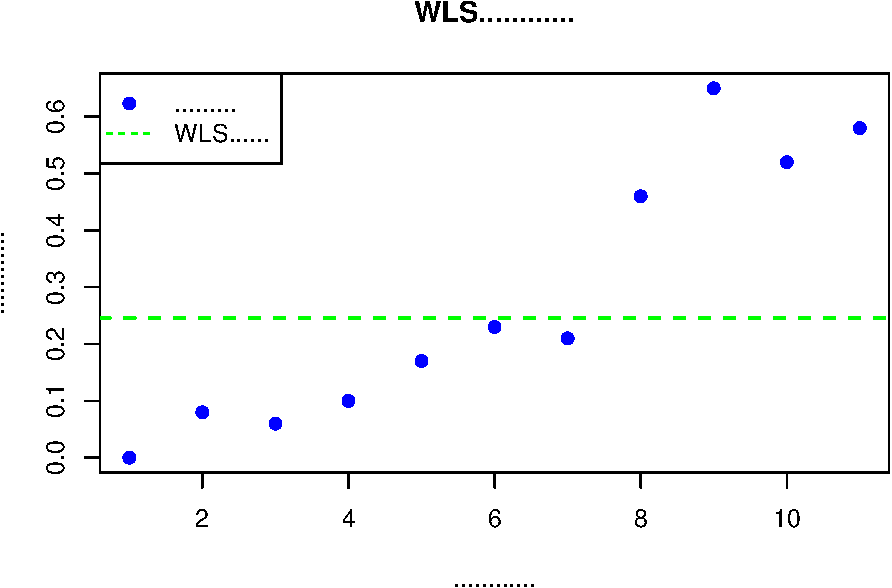
\includegraphics{未命名_files/figure-latex/unnamed-chunk-4-1.pdf}

\begin{center}\rule{0.5\linewidth}{0.5pt}\end{center}

\hypertarget{ux52a0ux6743ux6b8bux5deeux4e0eux6a21ux578bux8bcaux65ad}{%
\subsection{5.
加权残差与模型诊断}\label{ux52a0ux6743ux6b8bux5deeux4e0eux6a21ux578bux8bcaux65ad}}

\hypertarget{ux52a0ux6743ux6b8bux5deeux7684ux89e3ux91ca}{%
\subsubsection{5.1
加权残差的解释}\label{ux52a0ux6743ux6b8bux5deeux7684ux89e3ux91ca}}

加权残差 \(r^*_i\)
是每个观测点的实际值与模型预测值之间的差异,残差的大小可以反映模型的拟合效果。公式如下:

\[
r^*_i = \sqrt{w_i}(y_i - \hat{\mu})
\]

\hypertarget{ux8ba1ux7b97ux52a0ux6743ux6b8bux5dee}{%
\subsubsection{5.2
计算加权残差}\label{ux8ba1ux7b97ux52a0ux6743ux6b8bux5dee}}

在R中,我们可以通过\texttt{resid()}函数提取WLS模型的加权残差。

\begin{Shaded}
\begin{Highlighting}[]
\CommentTok{\# 提取加权残差}
\NormalTok{wls\_residuals }\OtherTok{\textless{}{-}} \FunctionTok{resid}\NormalTok{(wls\_model)}

\CommentTok{\# 打印加权残差}
\FunctionTok{print}\NormalTok{(wls\_residuals)}
\end{Highlighting}
\end{Shaded}

\begin{verbatim}
##           1           2           3           4           5           6           7           8           9          10          11 
## -0.24576389 -0.16576389 -0.18576389 -0.14576389 -0.07576389 -0.01576389 -0.03576389  0.21423611  0.40423611  0.27423611  0.33423611
\end{verbatim}

\hypertarget{ux6807ux51c6ux5316ux6b8bux5deeux4e0eux6760ux6746ux503c}{%
\subsubsection{5.3
标准化残差与杠杆值}\label{ux6807ux51c6ux5316ux6b8bux5deeux4e0eux6760ux6746ux503c}}

标准化残差可以将残差标准化,使其易于比较。通过\texttt{hatvalues()}函数计算杠杆值,可以识别对模型影响较大的观测点。

\begin{Shaded}
\begin{Highlighting}[]
\CommentTok{\# 计算杠杆值(hat values)和标准化残差}
\NormalTok{wls\_hat\_values }\OtherTok{\textless{}{-}} \FunctionTok{hatvalues}\NormalTok{(wls\_model)}
\NormalTok{wls\_standardized\_residuals }\OtherTok{\textless{}{-}}\NormalTok{ wls\_residuals }\SpecialCharTok{/} \FunctionTok{sqrt}\NormalTok{(}\DecValTok{1} \SpecialCharTok{{-}}\NormalTok{ wls\_hat\_values)}

\CommentTok{\# 打印标准化残差}
\FunctionTok{print}\NormalTok{(wls\_standardized\_residuals)}
\end{Highlighting}
\end{Shaded}

\begin{verbatim}
##           1           2           3           4           5           6           7           8           9          10          11 
## -0.25766989 -0.17697511 -0.19329326 -0.15989858 -0.07854004 -0.01652757 -0.03764041  0.21753420  0.42114868  0.28788795  0.34909823
\end{verbatim}

\hypertarget{ux56deux5f52ux8bcaux65ad}{%
\subsubsection{5.4 回归诊断}\label{ux56deux5f52ux8bcaux65ad}}

R提供了丰富的诊断工具,用于评估模型的拟合质量。通过\texttt{plot()}函数,我们可以生成回归诊断图。

\begin{Shaded}
\begin{Highlighting}[]
\CommentTok{\# 生成回归诊断图}
\FunctionTok{par}\NormalTok{(}\AttributeTok{mfrow=}\FunctionTok{c}\NormalTok{(}\DecValTok{2}\NormalTok{,}\DecValTok{2}\NormalTok{))}
\FunctionTok{plot}\NormalTok{(wls\_model)}
\end{Highlighting}
\end{Shaded}

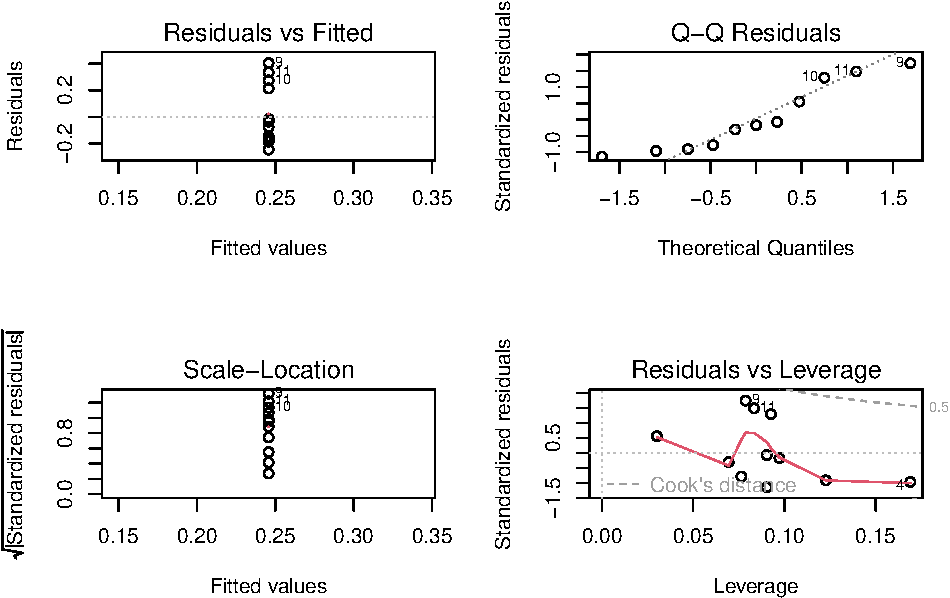
\includegraphics{未命名_files/figure-latex/unnamed-chunk-7-1.pdf}

\begin{center}\rule{0.5\linewidth}{0.5pt}\end{center}

\hypertarget{ux5e3dux5b50ux77e9ux9635hat-matrixux4e0eux6760ux6746ux503c}{%
\subsection{6. 帽子矩阵(Hat
Matrix)与杠杆值}\label{ux5e3dux5b50ux77e9ux9635hat-matrixux4e0eux6760ux6746ux503c}}

\hypertarget{ux5e3dux5b50ux77e9ux9635ux7684ux89e3ux91ca}{%
\subsubsection{6.1
帽子矩阵的解释}\label{ux5e3dux5b50ux77e9ux9635ux7684ux89e3ux91ca}}

帽子矩阵 \(H\) 是将观测值 \(Y\) 投影到模型拟合值 \(\hat{Y}\)
上的矩阵。加权线性回归的帽子矩阵定义为:

\[
H = X (X^T W X)^{-1} X^T W
\]

其中 \(W\)
是对角权重矩阵,帽子矩阵的对角元素称为\textbf{杠杆值(leverage)},用于衡量观测点对模型拟合的影响。

\hypertarget{ux6760ux6746ux503cux7684ux8ba1ux7b97}{%
\subsubsection{6.2
杠杆值的计算}\label{ux6760ux6746ux503cux7684ux8ba1ux7b97}}

通过\texttt{hatvalues()}函数,我们可以计算每个观测点的杠杆值,并识别那些对模型拟合影响较大的点。

\begin{Shaded}
\begin{Highlighting}[]
\CommentTok{\# 计算杠杆值}
\NormalTok{leverage }\OtherTok{\textless{}{-}} \FunctionTok{hatvalues}\NormalTok{(wls\_model)}

\CommentTok{\# 打印杠杆值}
\FunctionTok{print}\NormalTok{(leverage)}
\end{Highlighting}
\end{Shaded}

\begin{verbatim}
##          1          2          3          4          5          6          7          8          9         10         11 
## 0.09027778 0.12268519 0.07638889 0.16898148 0.06944444 0.09027778 0.09722222 0.03009259 0.07870370 0.09259259 0.08333333
\end{verbatim}

\begin{center}\rule{0.5\linewidth}{0.5pt}\end{center}

\hypertarget{ux603bux7ed3}{%
\subsection{7. 总结}\label{ux603bux7ed3}}

通过本R教程,我们详细介绍了普通最小二乘法(OLS)和加权最小二乘法(WLS)的基本概念及其在R中的实现。我们展示了如何计算残差、标准化残差和杠杆值,解释了加权线性回归模型中各个观测点对拟合的影响。

加权线性回归是一种强大的工具,特别适用于解决数据中存在异方差性的问题。通过为不同观测点赋予不同权重,WLS能够提高模型的拟合效果,确保估计的可靠性。

\end{document}
